%!TEX root = ../crimson_throne_book_main.tex
% 2014-08-14
After some quick healing the companions enter the tumulus into which the burly bugbear disappeared. Quint supplies some much needed light with a simple spell cast on his buckler. A tunnel leads under the hill, immediately splitting off in three directions. A quick examination of the left and right passage reveals two round rooms, where the moisture in the walls has worn away any marking that might have once adorned them. The chamber to the right is being used as a private bedroom with some hides on the ground and a makeshift shrine of old bones and skulls; the room to the left has a big hole in the ground which serves as a waste pit and toilet.\\

The main tunnel leads deeper into the tumulus and provides access to the ancient burial chamber, with eight alcoves lining the walls. Four bugbears are waiting for the heroes in here, one of which has taken up position on a stone table in the middle of the room. He forms the perfect target for Jasan's first arrow, which kicks off the fight. A bugbear in the back of the room seems to master some magic and reacts by casting a spell on Balian. The ranger feels his breastplate growing hotter, but Sjo's quick thinking provides the perfect 'antidote' for his scorching {\itshape heated metal} in the form of  {\itshape resist energy} . Quint demoralizes the opponents with another  {\itshape satirical} performance, while Puk jumps into the fray on top of a barrel. His tiny blade does not penetrate his adversary's armor, but the halfling has put himself in a precarious position, taking two firm hits from the bugbears that face him. Balian and his dog Spyder also charge forward, but their attacks go wide. Despite his fierce growls and sharp teeth, the canine is no match for the bugbear leader, who steps in and mercilessly hammers the dog with two main hand hits and one off-hand swing. His morningstar and light hammer drip with blood as the dog drops to the floor. This hulking creature delivers a mean punch, Sjo understands. His  {\itshape hold person} outside the entrance on this brute was even more valuable than he realized. He tries the spell again, but this time the hairy beast resists his magic. Meanwhile Balian draws his first blood of the fight by cleaving through the two bugbears that are pressing Puk. The halfling cannot get into an advantageous position without putting himself in even more risk and takes a defensive stand, which makes his opponents miss their attacks. In the meantime Jasan fires another arrow in the bugbear on the stone table, who just received some healing from the druid in his back.\hyperref[fig:Shoanti-tumulus-475539806]{ With Spyder down, Balian is now the leader's next target } : the hulk steps forward and pummels the ranger twice with his morningstar, reserving his backhand swing for Quint. The creature snorts out a hysteric laugh to celebrate his success. Quint feels that it is high time to swing the momentum of the fight and decides to use another of his tricks. He pulls out his whip and lashes it around the ankles of the bugbear on the table, pulling the creature's legs out from under him. Balian interrupts its attempt to rise with a deadly strike and takes its place on the stone table, finally gaining a flank with Puk on the other bugbear. The halfling takes full advantage of this position and pulls out two vicious sneak attacks that cut the unfortunate mutt down. At last the battle seems to turn for the better. Sjo engages the druid, who pulls out a sickle that glances off the Shoanti's plate. The fire-wielding healer retorts by spewing forth a sheet of flames that scorches both enemies that are left standing. Still, the fierce bugbear leader does not give up and continues bashing Sjo and Quint. He also proves to be very hard to hit, so the fight  {\itshape ain't over yet} . Sjo uses heroic inspiration (we use hero points)  {\itshape hold person} , but again the towering monster resists. Next Quint also fails to trip him. Puk and Balian now flank the creature, but the halfling cannot get through its defenses. Balian fares better and cuts deeply into its flesh. The ranger continues the arc of his blade and slices through the druid as well. Despite the bleeding gash, the leader seems unimpressed and pushes the attack, wounding Balian, Puk and Quint with his whirling weapons. A second attempt by Quint to topple the bugbear champion succeeds, leaving the being prone between the bloodthirsty halfling, the fuming Shoanti and the enraged ranger. The companions exploit the opportunity to the fullest, literally hitting their enemy while he's down. Balian hacks heavily into the hulk's frame and Puk's flashing blades finally finish the brute off. The druid is helpless against superior numbers and swiftly follows his brethren to the grave. \\

\begin{figure}[h]
	\centering
	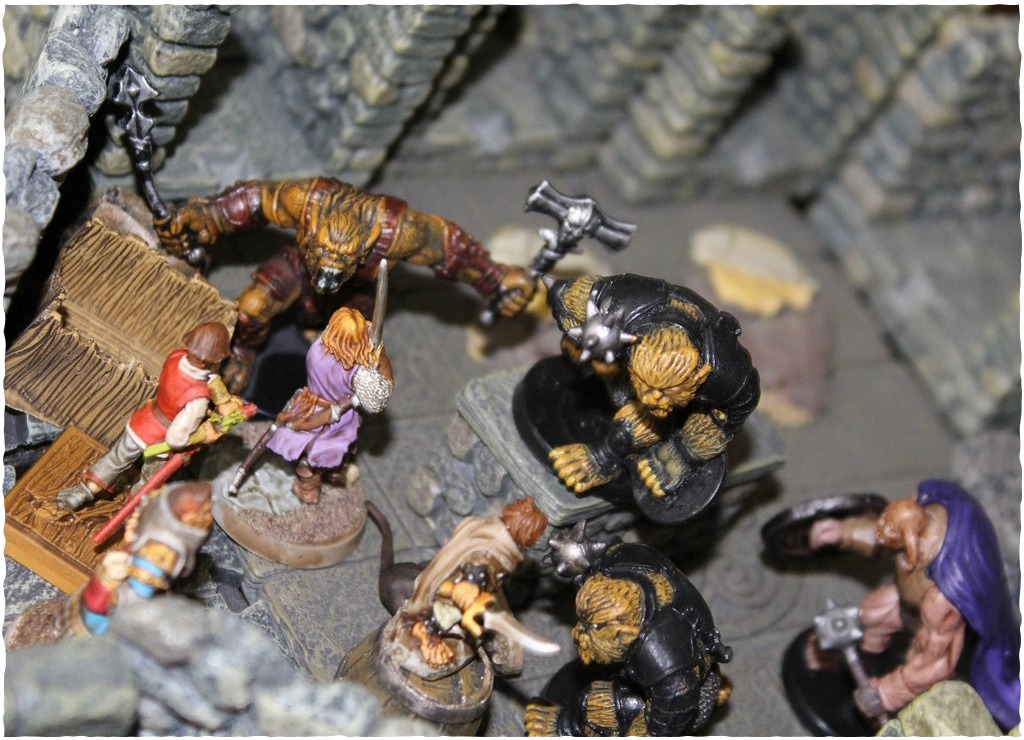
\includegraphics[width=0.4\textwidth]{images/Shoanti-tumulus-475539806_mod.jpg}
	\caption{Shoanti tumulus}
	\label{fig:Shoanti-tumulus-475539806}
\end{figure}

The companions take a few moments to catch their breath. As they are healing up, two young voices call out from one of the alcoves that has been blocked by a heap of stones. Farmer Barold's sons, Vern and Sender, have been locked up there. They are overjoyed when their rescuers inform them that both their father and cow Bianca are still alive. Puk leads the search of the complex and unearths a hefty pouch with gold, while Quint discovers that the bugbear leader's studded leather is magical and Sjo finds an old Shoanti pendant around the druid's neck. The engraved runes spell {\itshape Storval ekbitel nalharest} , which is Shoanti for  {\itshape We walk the land as brothers} . Other markings in the stone table identify this tomb as a Shundar-Quah grave, another of the Shoanti tribes that once roamed this country. Sjo is disgusted at the bugbear sacrilege of this holy place and asks his friends to help him remove them from the tumulus. The companions drag the cadavers of their enemies outside and build a funeral pyre. They also take out the bugbears' supplies from the tumulus and give them to Barold, along with 100 gold sails from the loot. This small gift is a true fortune for the simple farmer, who is very grateful for the safe return of his children, his cow Bianca and the heroes' generosity. It is already a few hours past noon when the companions head back to Korvosa. Fortunately they now have horses, so they should be able to make up for the time they lost.\\

